\documentclass[conference]{IEEEtran}
\IEEEoverridecommandlockouts
% The preceding line is only needed to identify funding in the first footnote. If that is unneeded, please comment it out.
\usepackage{cite}
\usepackage{hyperref}
\usepackage{makecell}

\usepackage{amsmath,amssymb,amsfonts}
\usepackage{algorithmic}
\usepackage{graphicx}
\usepackage{textcomp}
\usepackage{xcolor}
\def\BibTeX{{\rm B\kern-.05em{\sc i\kern-.025em b}\kern-.08em
    T\kern-.1667em\lower.7ex\hbox{E}\kern-.125emX}}
\begin{document}

\title{Dynamic LION*\\
{\footnotesize \textsuperscript{*}LION: Empowering Multimodal Large Language Model with Dual-Level Visual Knowledge}
% \thanks{Identify applicable funding agency here. If none, delete this.}
}

\author{
  \IEEEauthorblockN{WooSeok Kim\IEEEauthorrefmark{1}\thanks{* These authors contributed equally to this work.}}
  \IEEEauthorblockA{\textit{Department of Computer Science} \\
  \textit{Carleton University}\\
  wooseokkim@cmail.carleton.ca}
  \and
  \IEEEauthorblockN{Nassim Tiraoui\IEEEauthorrefmark{1}}
  \IEEEauthorblockA{\textit{dept. name of organization (of Aff.)} \\
  \textit{Ottawa University}\\
  ntira053@uottawa.ca}
} 

\maketitle

\begin{abstract}
In the past few years, Multimodal Large Language Models (MLLMs) have shown strong potential in expanding the modalities that the LLMs can process.
The performance of LLMs with multimodal data continues to improve by leveraging the knowledge between modalities.
One recent work, the dual-\textit{L}evel v\textit{I}sual kn\textit{O}wledge e\textit{N}hanced Multimodal Large Language Model (LION), demonstrates improvements over existing MLLMs in visual knowledge.
One of the most known issues with vision models is an insufficient extraction and reasoning of visual knowledge.
LION tackles this issue by incorporating visual knowledge through the progressive integration of fine-grained spatial-aware features and the use of soft prompting with high-level semantic visual evidence.
Despite these advancements, the soft prompting technique remains the need for an exploration.
As mentioned from the LION paper, soft prompting method still has the danger from hallucination to some degree.
In this report, we propose a dynamic soft prompting to mitigate the object hallucination problem, and explore its effectiveness.
\end{abstract}

\begin{IEEEkeywords}
Multimodal Large Language Model (MLLM), LLM, Vision Encoder
\end{IEEEkeywords}

\section{Introduction}
Recent research \cite{kuang2025natural} shows an increasing use of Multimodal Large Language Models (MLLMs) with its ability to incorporate different types of knowledge across various modalities (\textit{i.e.}, image and text).
This is especially useful for vision language (VL) tasks, such as reasoning of the input image using natural language style knowledge.
Nevertheless, there still exists limitations of extracting and reasoning of visual knowledge.
This is largely due to most of the existing MLLMs employ vision encoder that was pretrained on a coarsely aligned image-text pairs, which ultimately leads to insufficient extraction of visual information.

One recent work, dual-\textbf{L}evel v\textbf{I}sual kn\textbf{O}wledge e\textbf{N}hanced Multimodal Large Language Model (LION) \cite{chen2024lion}, mitigates the issue by progressively incorporates fine-grained spatial-aware visual knowledge and applies soft prompting of high-level semantic visual envidence.
Specifically, the authors propose a stage-wise instruction-tuning strategy to perform image-level and region-level VL tasks.
As shown in Fig.~\ref{fig:overview}, it learns the visual knowledge separately by using two different adapters, and then a router module is used to aggregate the knowledge from image-level and region-level adapters into a single vision knowledge representation.
In addition, LION employs a very well-known foundation model, Recognize Anything Model (RAM) \cite{ram}, as a vision extractor to obtain image tags off-the-shelf.
Tags extracted from RAM are used to generate a soft prompt, which is the key component of the paper.
A soft prompt is an instruction template with image tags and trainable parameters representing the prompt.
The authors suggest the template as such,
\textit{``According to \textless hint\textgreater, you are allowed to use the following tags:''},
where the \textit{\textless hint\textgreater} will be replaced with a trainable soft prompt, and the tags from RAM will be inserted at the end of the template.
In this way, the model can avoid potential negative influence by the imperfect predictions from RAM.

\begin{figure*}
  \centerline{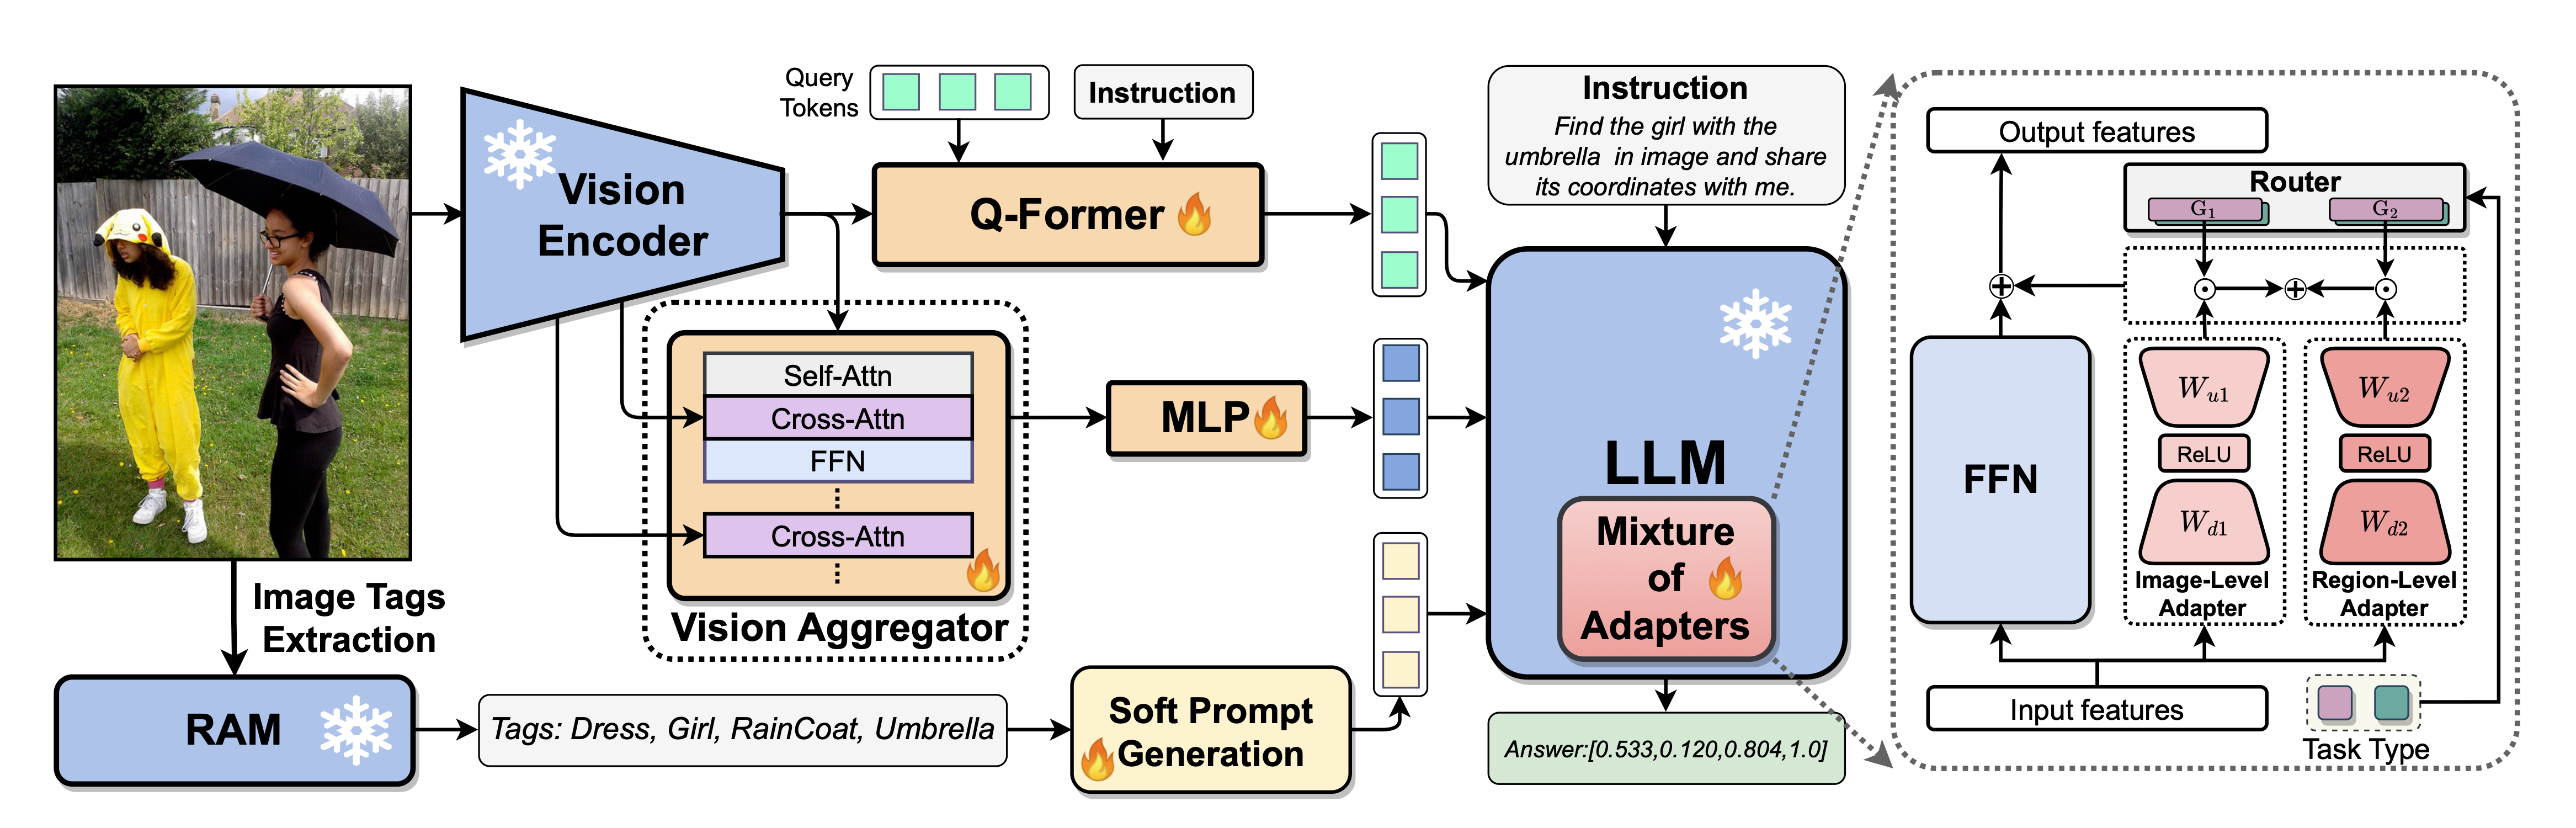
\includegraphics[width=\textwidth]{imgs/lion_overview.png}}
  \caption{Overview of the original LION \cite{chen2024lion}. The model extracts visual features from Q-Former, and combines them with fine-grained spatial-aware features from the vision aggregator. The Mixture-of-Adapters with a router in the frozen LLM dynamically fuses visual knowledge learned from different visual branches and LLM adapters based on the task types (image-level and region-level).}
  \label{fig:overview}
\end{figure*}

\section{Limitations of the Previous Work}\label{limits}

While LION achieves high performance in image captioning, visual question answering (VQA), and visual grounding tasks, object hallucination is one of the most concerned issue from the paper, as the authors mentioned.
This challenge is due to an imperfect vision model, such as RAM, generating false visual knowledge and passing it to other modalities.
Because of this MLLM's high dependency to the vision model's performance, potential object hallucination problem is inevitable.

Not only does the performance of off-the-shelf vision models contribute to the problem, but over-reliance on statistical bias \cite{hal_bias} and unimodal priors \cite{unimodal_bias, unimodal_2} can also lead to challenges such as visual hallucinations.
This shows that the challenge stems from the MLLM's systemic nature, in which its purpose is to find correlations between modalities and align various knowledge into a unified knowledge.
Nevertheless, MLLMs with foundation models are still considered to be the mainstream \cite{foundationMLLM}, due to their high performance and ease of implementation.


\section{Related Work}
As discussed from Section~\ref{limits}, extracting visual features for MLLMs is especially challenging.
This is heavily due to the misalignment between text and image pairs, leading the MLLMs' unexpected performance \cite{cho2022fine, jain2024vcoder}.
Since it relies heavily on the dataset being used, recent works focus to utilize the text and image pairs in order to capture fine-grained visual features.
NoteMR \cite{fang2025guided} utilizes knowledge notes and visual notes for reducing object hallucination.

Y.~Zeng \textit{et al.}~\cite{contrastive} fine-grained contrastive learning

\subsection{Soft Prompting}

The IEEEtran class file is used to format your paper and style the text. All margins, 
column widths, line spaces, and text fonts are prescribed; please do not 
alter them. You may note peculiarities. For example, the head margin
measures proportionately more than is customary. This measurement 
and others are deliberate, using specifications that anticipate your paper 
as one part of the entire proceedings, and not as an independent document. 
Please do not revise any of the current designations.

\section{Method}
Before you begin to format your paper, first write and save the content as a 
separate text file. Complete all content and organizational editing before 
formatting.
proofreading, spelling and grammar.

\subsection{Model Architecture}\label{model_architecture}

\begin{figure}
  \centerline{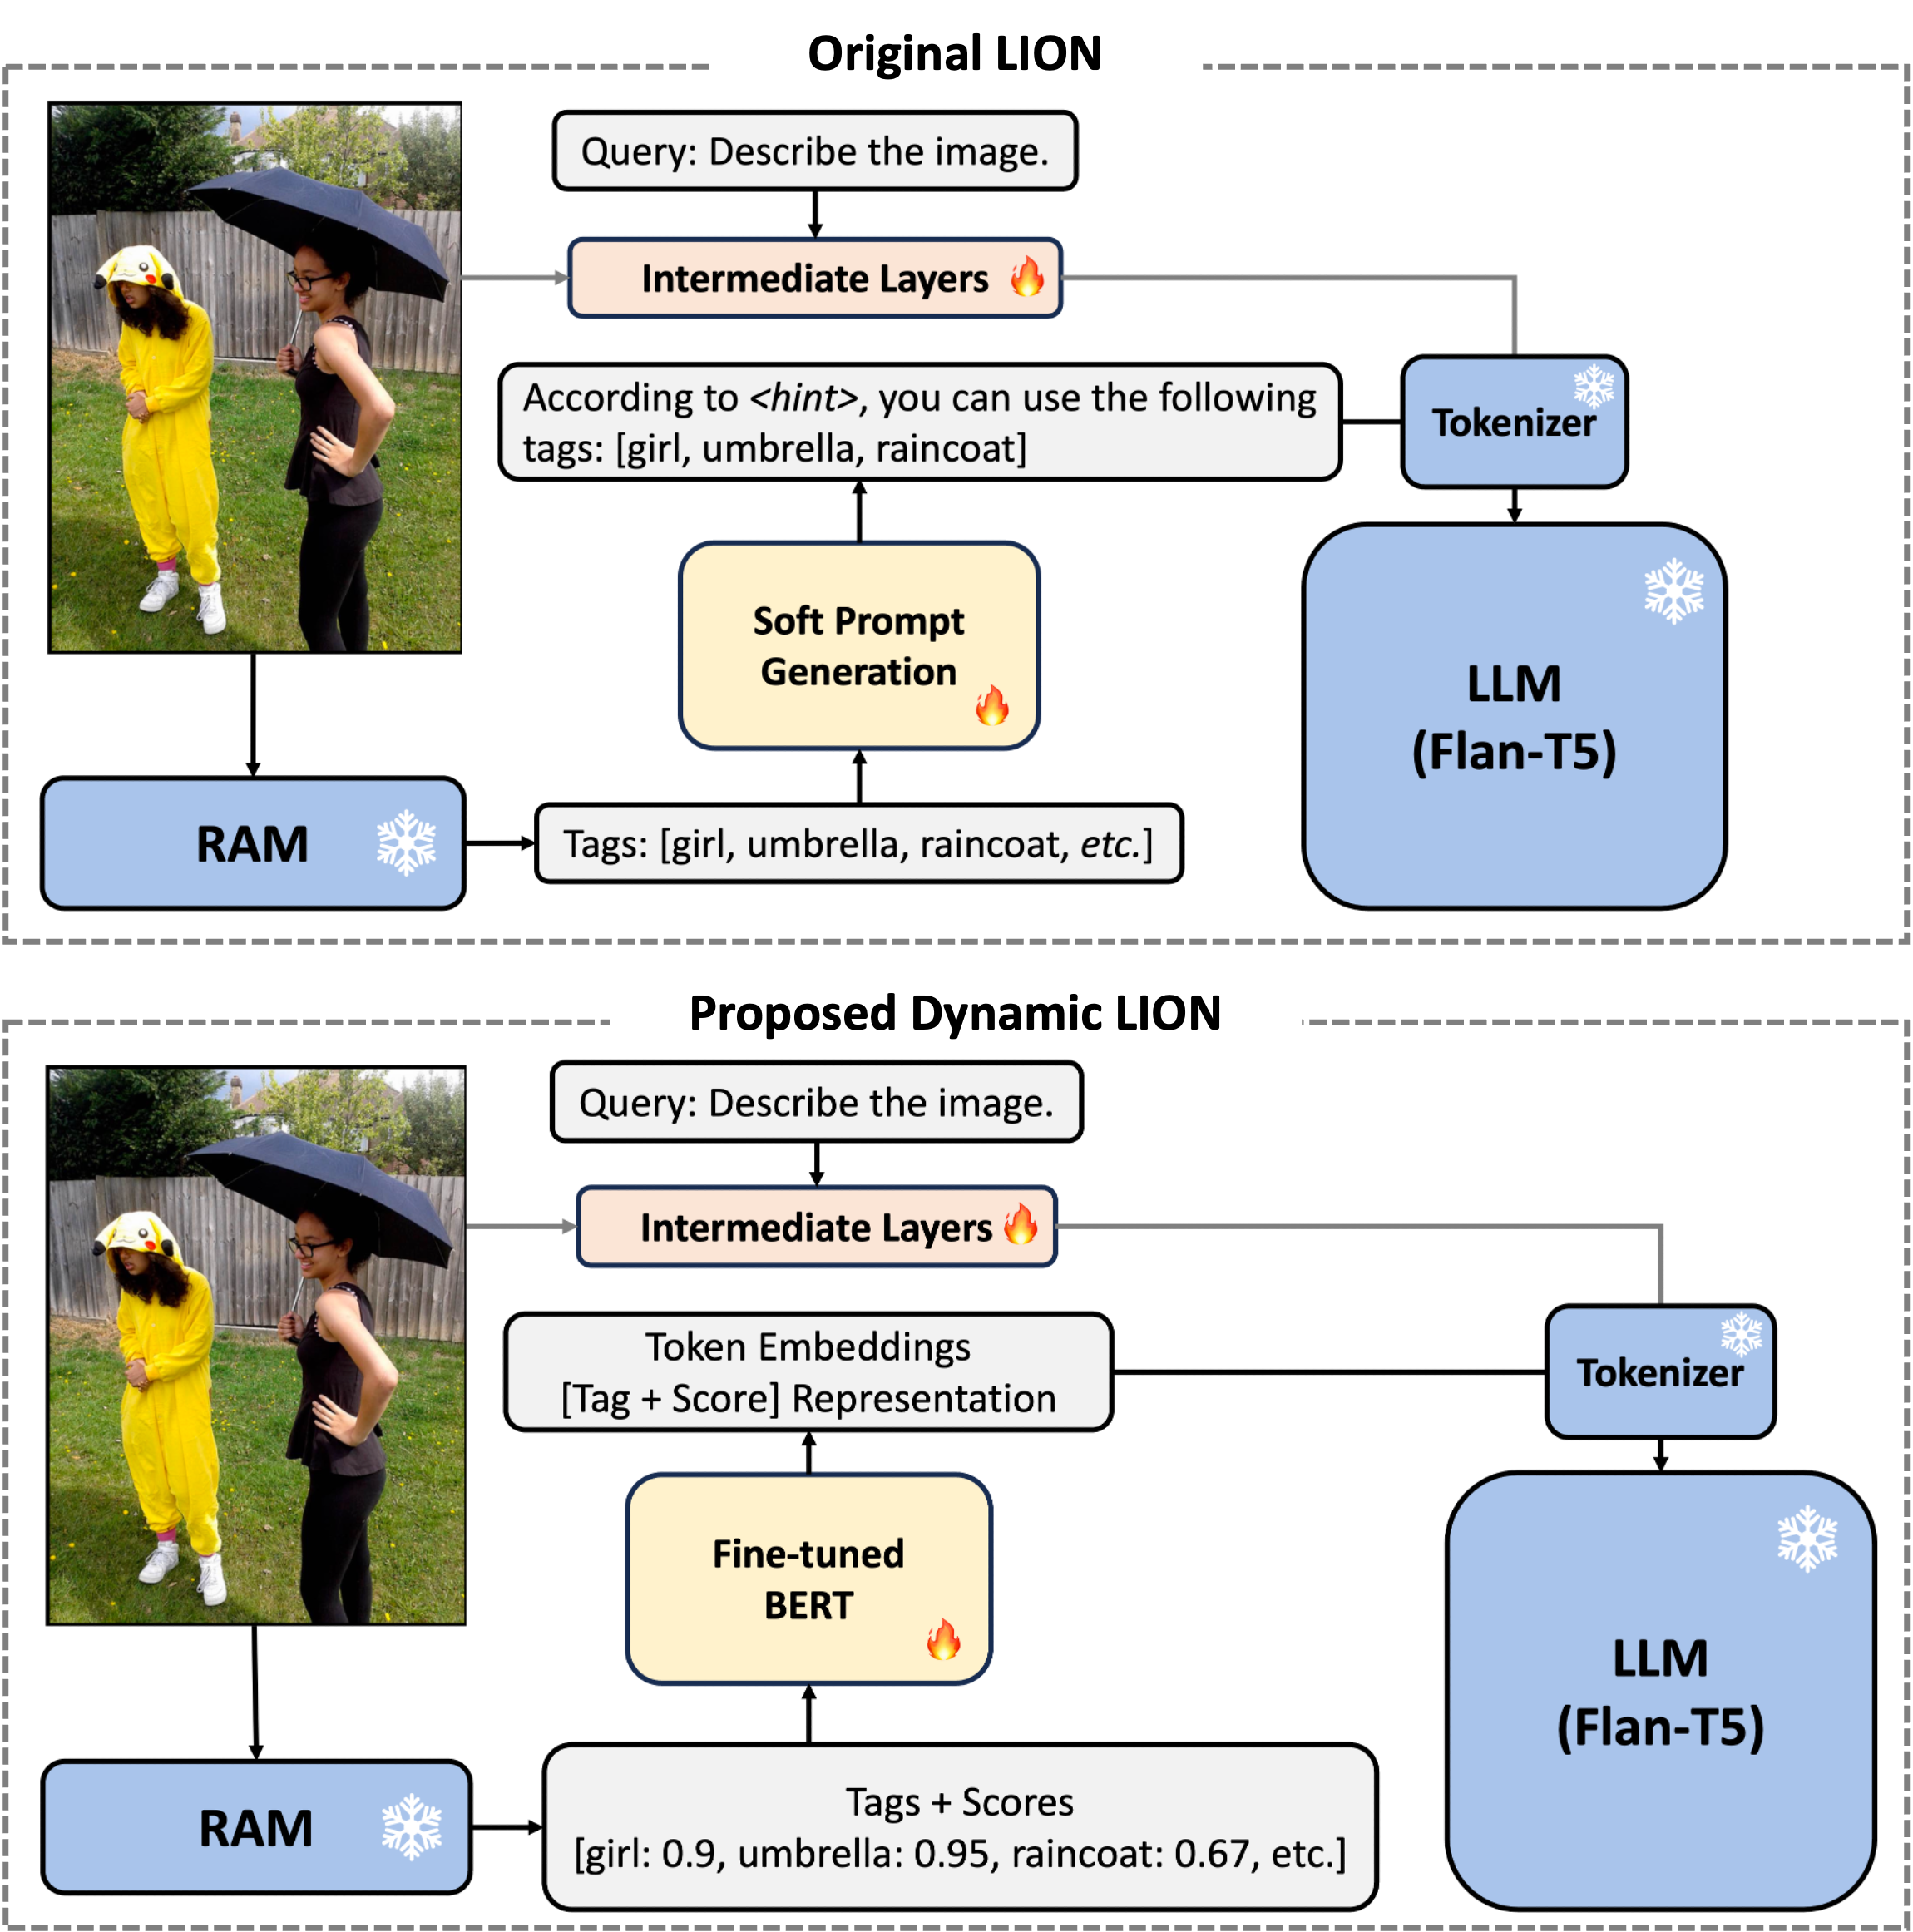
\includegraphics[width=\linewidth]{imgs/prompting.png}}
  \caption{Comparison between the original LION's soft prompting and the proposed dynamic soft prompting. Original soft prompting uses image tags and trainable vector (\textit{hint}), and dynamic soft prompting uses fine-tuned BERT model to generate token embeddings, given the tags and confidence scores.}
  \label{fig:soft_prompt_comp}
\end{figure}


\section{Experiments}

In this section, we present experiments including fine-tuning the BERT model for dynamic soft prompting, LION's overall training results, image-level task evaluation, and region-level task evaluation.
Due to an hardware issue, we have tested the LION model with the smallest LLM model, namely Flan-T5-small.
We trained our proposed model with NVIDIA RTX 4070 TI GPU with 16GB memory.
It uses Parameter-Efficient-Fine-Tuning (PEFT) learning rate scale of 5.0.
The training took 10 epochs, and validate every epoch.

\subsection{Fine-tuning BERT}

As discussed from Section~\ref{model_architecture}, dynamic soft prompting requires fine-tuning process of the BERT model.
The purpose of this fine-tuning is to align image captions with the given image, since most of the hallucination issues arose from the misalignment of image-text pairs.
To prevent the aforementioned issue, triplet margin loss is employed which requires anchor, positive, and negative pairs.
We use MS-COCO \cite{mscoco} to fine-tune the BERT model, using all five captions per image.
For an anchor, RAM generates tags and confidence scores for each tag, and the token embeddings fof these tags and scores will used as an anchor from the BERT model.
For positive, token embeddings of image captions are used.
To be more specific, all five image captions from MS-COCO are fed to Sentence Transformer \cite{all-mpnet-base-v2} to transform them into token embeddings.
Then, each token embeddings are compared with the one represents the five image captions which was made by averaging all five token embeddings.

As shown in Fig.~\ref{fig:bert_finetune}, the learning curve shows that the BERT model is successfully fine-tuned with tokenizing image tags and confidence scores with respect to MS-COCO image captions.
The training loss and validation loss are decreasing gradually in a same manner, showing low loss values.

Not only does the loss is decreasing, the cosine similarity plot shows that the BERT model is actually producing an output where it is alike with positive image caption but differentiating negative image caption.
This allows BERT to generate token embeddings implying image tags with image captions for dynamic soft prompt in LION.

\begin{figure}
  \centerline{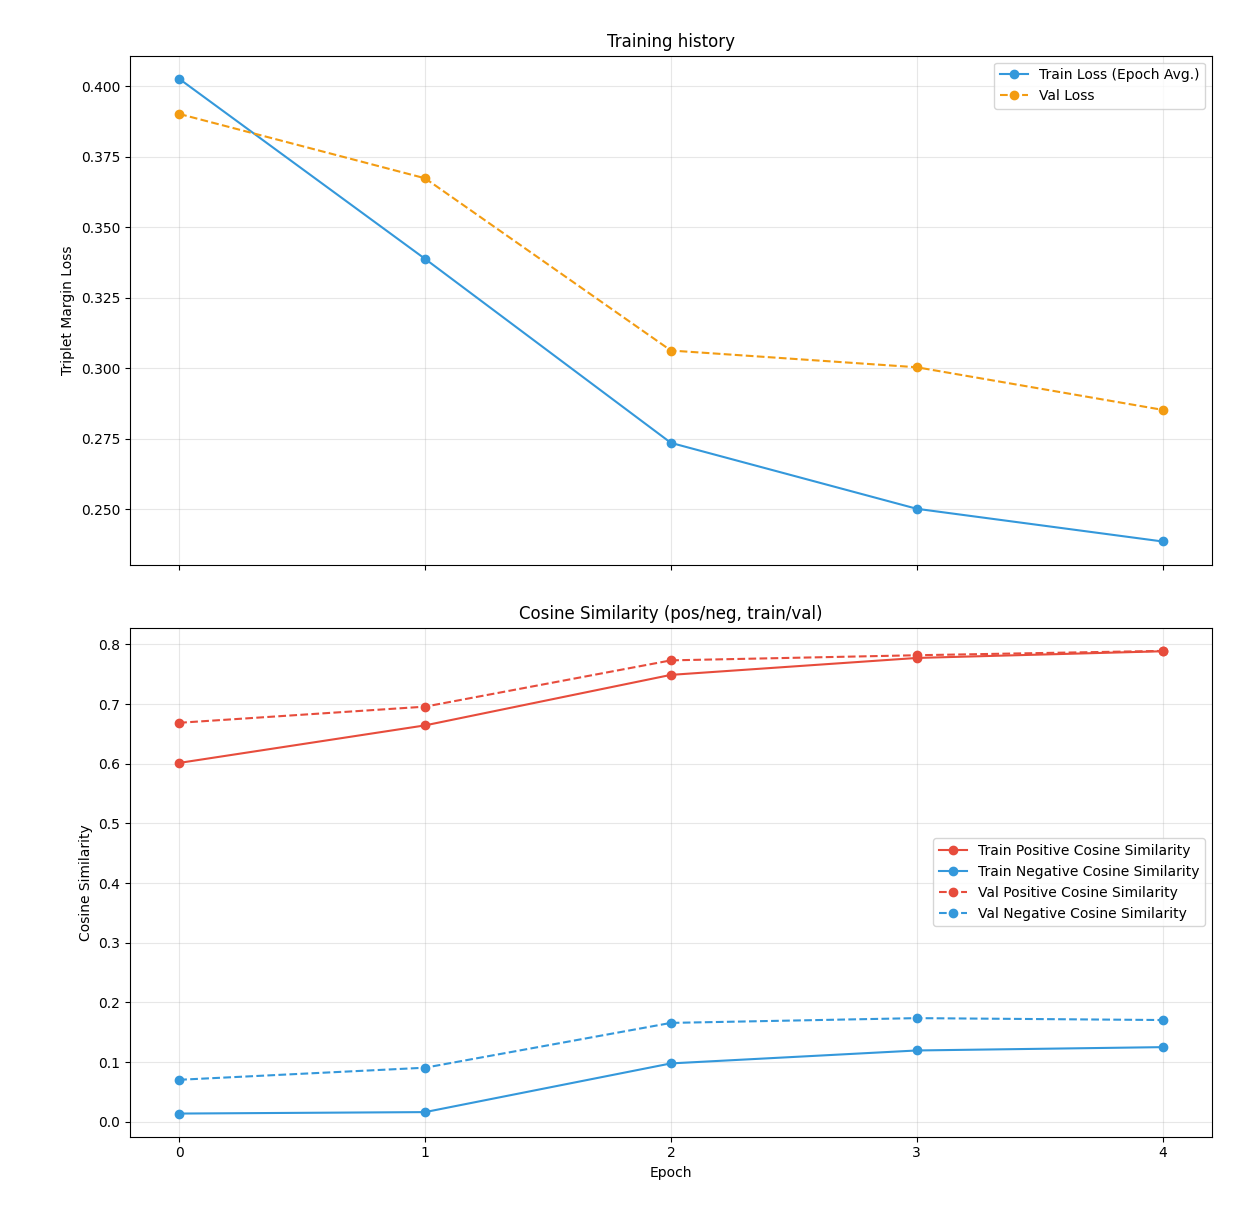
\includegraphics[width=\linewidth]{imgs/cosine.png}}
  \caption{Fine-tuning result of BERT model usded for dynamic soft prompt generation. (Top) Both the training and validation triplet margin loss gradually decrease, showing its convergence. (Bottom) Cosine similarity scores measured from training and validation set, differentiating positives and negatives.}
  \label{fig:bert_finetune}
\end{figure}

\subsection{Training Result of LION with Dynamic Soft Prompt}

With the use of fine-tuned BERT for dynamic soft prompt, Dynamic LION is trained then evaluated with the original LION.

\begin{figure}
  \centerline{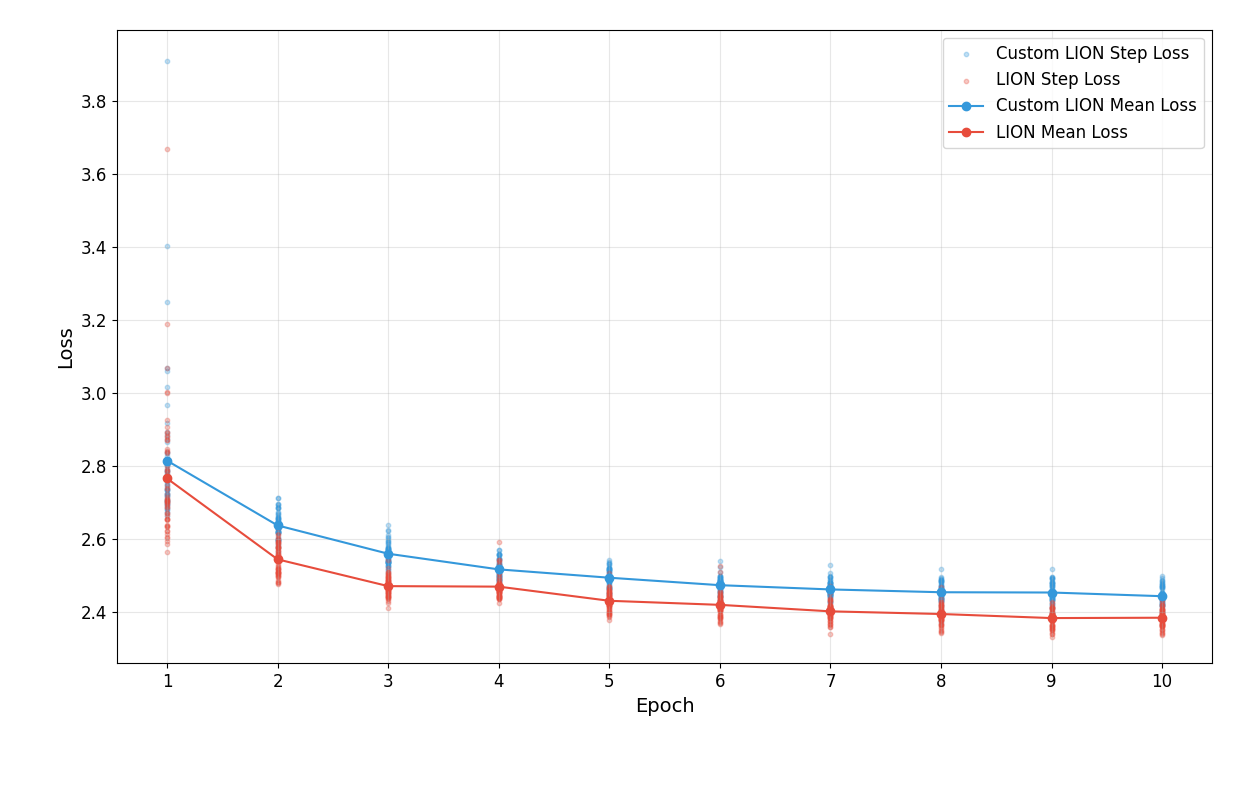
\includegraphics[width=\linewidth]{imgs/loss_converge.png}}
  \caption{Training loss curves for the original LION model (red) and the custom LION with dynamic soft prompting (blue). While the original LION achieves slightly lower loss throughout training, both models follow nearly identical learning trajectories.}
  \label{fig:loss_comp}
\end{figure}

\subsection{Evaluations on Image-Level VL Tasks}

We evaluate the dynamic soft prompting method's performance on two types of image-level VL tasks, which are image captioning and VQA.
For image captioning, COCO caption \cite{cococap} and TextCaps \cite{textcaps} datasets are used, and report CIDEr as the evaluation metric.
Also for VQA task, OKVQA \cite{okvqa} and AOKVQA \cite{aokvqa} datasets are used, and its performance is measured by Top-1 Accuracy metric.

The models used for the comparison are denoted as LION-4B, LION-12B, LION-small, and custom LION-small (ours).
Each model is based off of a Flan-T5 model with different sizes of parameters. 
LION-4B and LION-12B are equipped with Flan-T5-XL (4B parameters) and Flan-T5-XXL (11B parameters), respectively.
LION-small and custom LION-small use the same LLM, the Flan-T5-small model (80M parameters).
Obviously, the higher the number of parameters the model has (\textit{i.e.}, LION-4B and LION-12B), the more likely the model is to perform better.
Our goal is to while outperform LION-small model, also achieve a certain level of performance comparable to LION-4B or even LION-12B.

As shown in Table~\ref{tab:image-level}, LION-4B and LION-12B achieves the best performance.


\begin{table}
  \centering
  \caption{Comparison of image captioning and VQA performance performance}
  \begin{tabular}{l|cc|cc}
    \Xhline{2\arrayrulewidth}
    Model & COCOCap & TextCaps & OKVQA & AOKVQA \\
    \hline\hline
    LION-small & 69.09 & 26.45 & 2.3\% & 1.8\% \\
    LION-small (ours) & 21.40 & 4.68 & 16.3\% & 11.3\% \\
    LION-4B & 138.20 & 104.87 & 51.08\% & 59.98\% \\
    LION-12B & 139.25 & 108.76 & 57.33\% & 60.87\% \\
    \Xhline{2\arrayrulewidth}
  \end{tabular}
  \newline
  \label{tab:image-level}
\end{table}


\subsection{Evaluations on Region-Level VL Task}

For region-level VL task, referring expression comprehession (REC) dataset, RefCOCO \cite{refcoco}, is used to evaluate the model's ability to locating target object.

\begin{table}
  \centering
  \caption{Comparison of REC performance on the RefCOCO}
  \begin{tabular}{l | c | c}
    \Xhline{2\arrayrulewidth}
    Model & RefCOCO (IoU 0.5) & RefCOCO (IoU 0.1) \\
    \hline \hline
    LION-small & 0\% & 7.3\% \\
    LION-small (ours) & 0 \% & 2.9\% \\
    LION-4B & 57.57\% & - \\
    LION-12B & 58.54\% & - \\
    \Xhline{2\arrayrulewidth}
  \end{tabular}
  \newline
  \label{tab:region-level}
\end{table}

\bibliography{ref.bib}
\bibliographystyle{IEEEtran}
\end{document}
